%Struktur
% -Festlegung von Software-Kriterien
% -Auswahl des Verfahrens
% -Reproduktion des Verfahrens aus der Literatur
% 	-Kantenerkennung
% 	-Segmentierung
%	-Probleme & besondere Erkenntnisse
% -Erweiterung des Verfahrens
%	-Grundlegende Änderungen des Verfahrens
%	-False edge removal
%	-Point marking and cloud filtering
%	-misc.


\chapter{Entwicklungsprozess der Software}
Die Rücksichtnahme des Einsatzzwecks bei der Design und Entwurf des Verfahrens sowie die Entwicklung der Software war erforderlich, um die gewünschte Funktionalitäten gewährleisten zu können. Das Verfahren soll Kanten und Geometrien nicht nur in vollständig generierten Punktwolken erkennen, sondern auch in unvollständige Punktwolken, die iterativ wachsen. Hierbei wird ein Laserliniensensor eine Kante eines Werkstücks oder Objektes entlang geführt und somit sequentiell abgetastet. Deswegen wird die räumliche Struktur des Objektes nicht in einer einzigen Aufnahme abgebildet, sondern durch mehrere kleine Einzelaufnahmen. Der intelligente Schweißroboter, der durch das Fraunhofer Institut für Produktions- und Automatisierungstechnik entwickelt wird, verwendet ein solches Verfahren zum Scannen eines Werkstückes und zur Erkennung Schweißnähte \autocite[39]{savla_intelligente_2022}. Mittels eines Lasersensors wird die Oberfläche des Werkstückes dreidimensional abgebildet. Aktuell wird eine Schweißkegelnaht durch die Erkennung der Schnittlinie zwei Ebenen markiert, die mittels RANSAC-Algorithmen auf die Punktwolke des Werkstückes gefittet werden. Dieses Verfahren zur Erkennung der Schweißnaht bietet allerdings kaum detaillierte Informationen über die Geometrie des Werkstückes an.\autocite[39-52]{savla_intelligente_2022}. Das, in dieser Arbeit entwickelte Verfahren soll das bestehende Verfahren ersetzen und somit seine Limitationen überwinden.

\begin{figure}[h]
	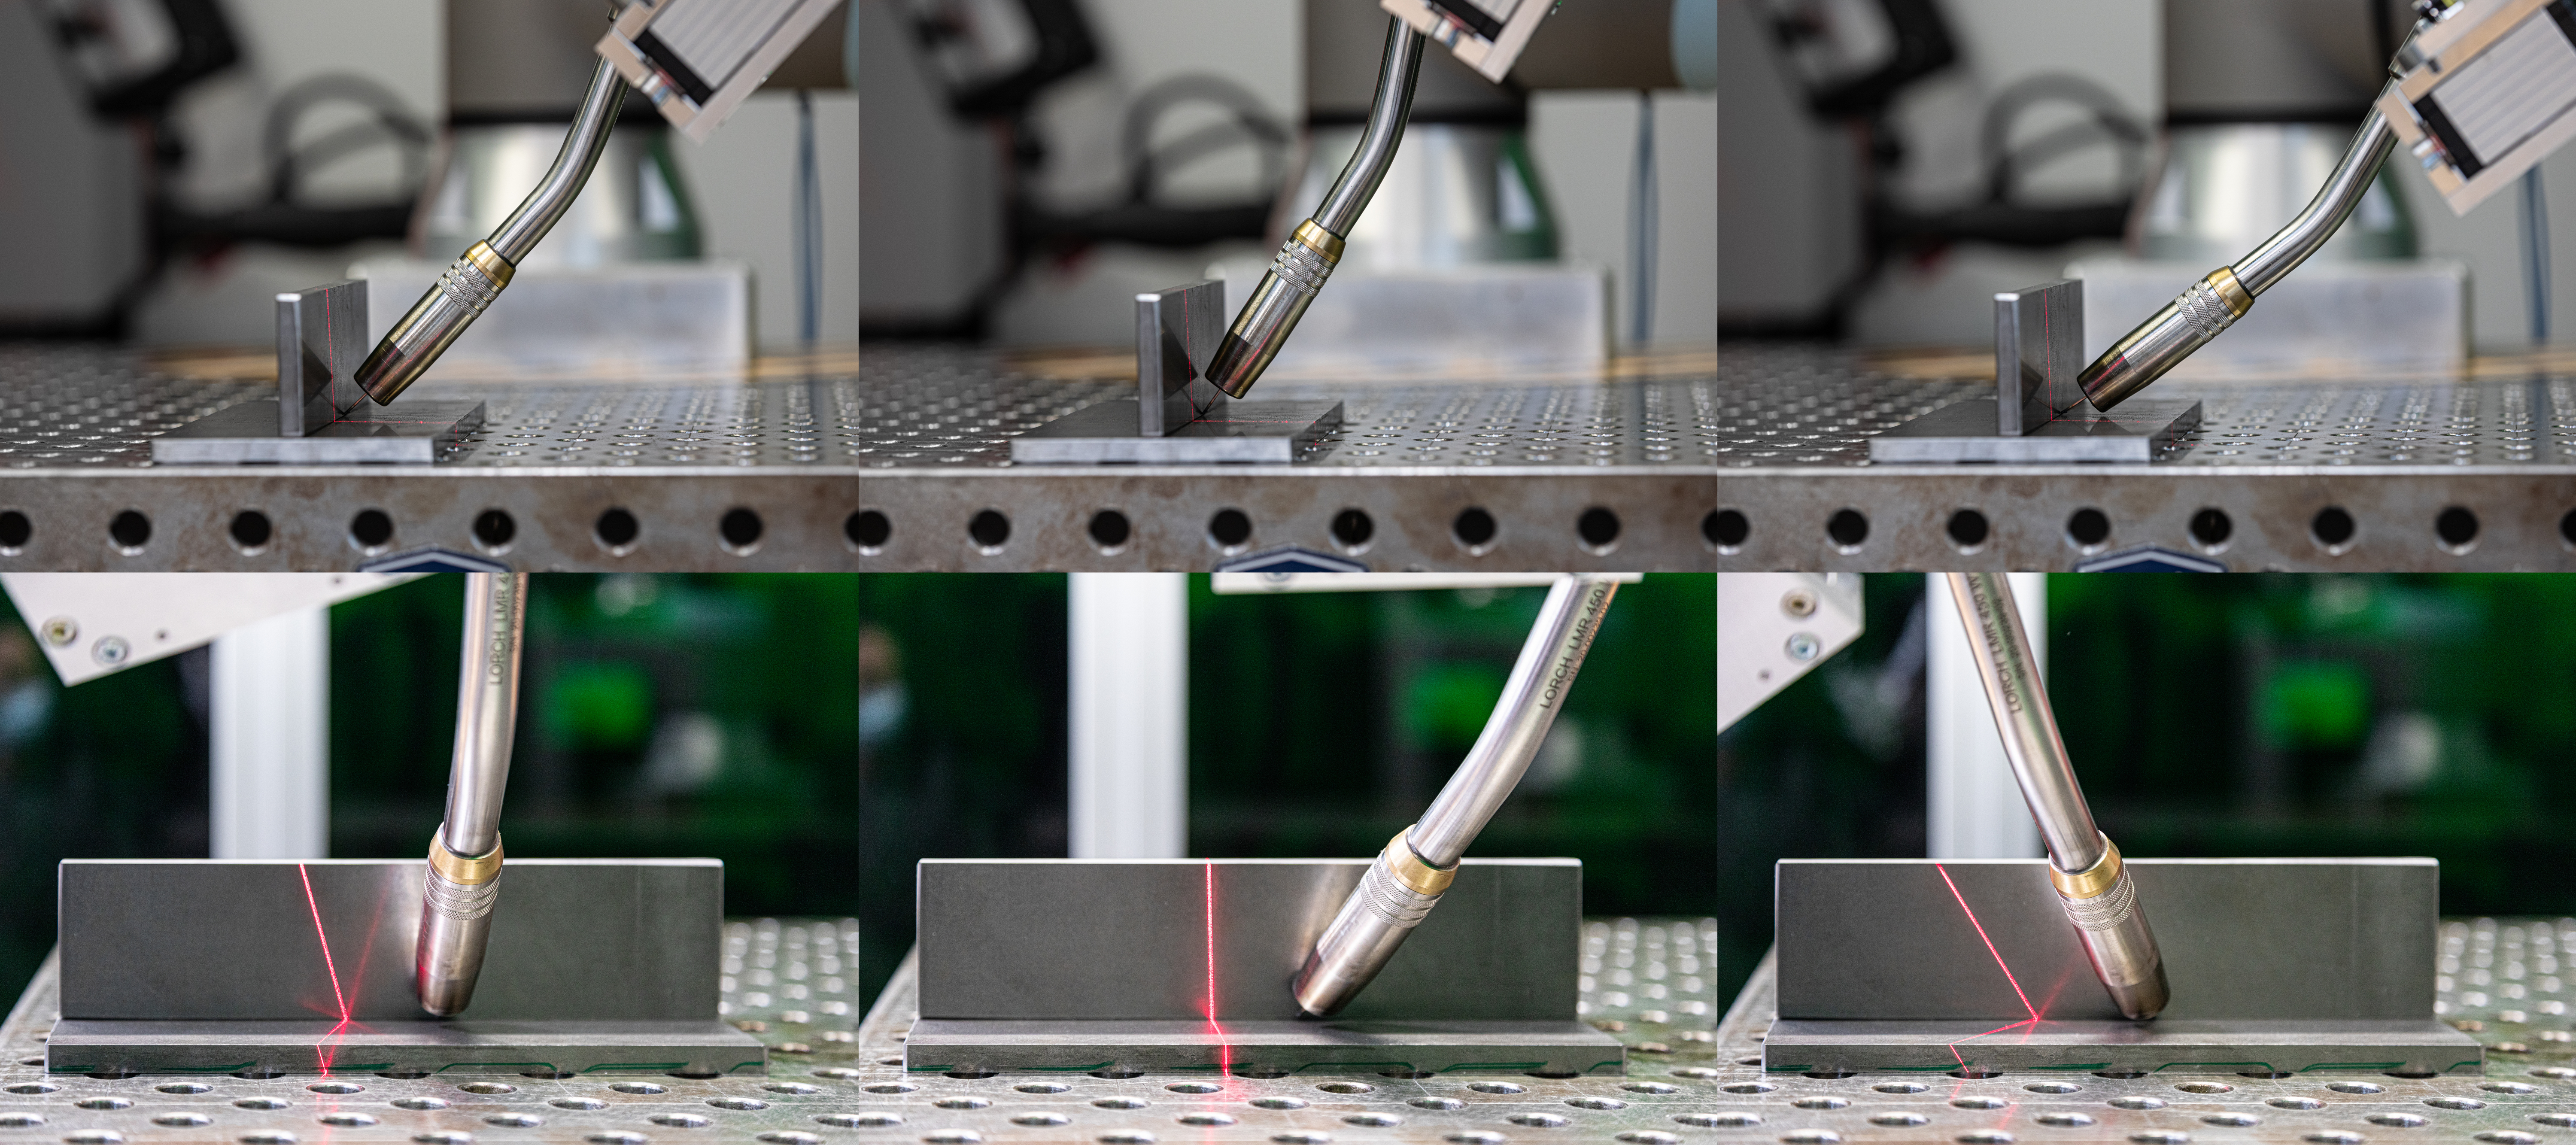
\includegraphics[width = \textwidth]{Abbildungen/collage.jpg}
	\centering
	\caption{Der Laserliniensensor} 
\end{figure}

\section{Vorbereitungen} \label{agpn_reproduction}
\subsection{Software-Voraussetzungen}\label{soft_voraus}
Bei der Auswahl eines geeigneten Verfahrens zur Detektierung Kanten in einer Punktwolke wurden einige Voraussetzungen festgelegt. Die Methode sollte in der Lage sein, nicht nur Außenkanten zu erkennen, sondern auch Innenkanten beziehungsweise Faltungen. Neben dem originellen Einsatzzweck sollte das Verfahren möglichst breit anwendbar sein und eine hohe Modularität aufweisen. Die Funktionen der Kantendetektierung und Punktesegmentierung sollten unabhängig von einander aufrufbar gestaltet werden, um dem Benutzer eine möglichst hohe Flexibilität anzubieten. Die Kantenerkennung sollte performant erfolgen und Punktwolken innerhalb eines praktischen Zeitraums verarbeiten. Letztlich soll das Programm in dem bestehenden Programmpaket des Schweißroboters integrierbar sein. Die Hardwarebeschleunigung des Verfahrens mittels eines Grafikprozessors wurde ausgeschlossen, da ihrer Verwendung mit dem Echtzeitkernels des Programmpakets zur Konflikte führt. 

\subsection{Auswahl eines Verfahrens}
Eine Literatursuche nach Verfahren zur adaptiven Erkennung von Kanten in wachsenden 3D Punktwolken für den Einsatzzweck ergab nichts. Die meisten Verfahren eigneten sich für die Kantenerkennung nur in vollständigen Punktwolken. Aus diesem Grund wurde die Entscheidung getroffen, ein vorhandenes Verfahren aus der Literatur zu wählen und es für den Einsatzzweck anzupassen. Drei unterschiedlichen Verfahren nach \textcite{bazazian_edc-net_2021}, \textcite{himeur_pcednet_2021} und \textcite{rachmadi_road_2017} zeigten viel versprechende Ergebnisse. Allerdings wurden neuronale Netze in dieser Verfahren verwendet, welches zu zwei Problemen geführt hätte. Aufgrund der Funktionsweise neuronaler Netze wäre es schwierig gewesen, diese für den Einsatzzweck ohne eine umständliche Anpassung des neuronalen Netzes anzupassen. Das zweite Hindernis entsteht durch die Einschränkung bei der Verwendung von Grafikprozessoren. Diese Prozessoren hätten die Rechenzeit neuronaler Netze sehr stark verringert und die schnelle Performanz des Verfahrens gewährleistet \autocite[625]{luo_artificial_2005}. Das numerische Verfahren nach \textcite{choi_rgb-d_2013} war auch für den Einsatzzweck ungeeignet, da es als Eingangsparameter eine RGB-D Datei erfordert. Somit wäre das Verfahren nur für eine Anwendung auf organisierten, gefärbten Punktwolken eingeschränkt. Es wurden zwei weitere Verfahren gefunden, die sich zur Erkennung Kanten in organisierten sowie unorganisierten Punktwolken eignen würden. \textcite{mineo_novel_2019} stellten eine numerische Methoden vor, welche zu einer hohen Genauigkeit Kanten erkennen konnte. Allerdings wurden keine Angaben über die Erkennung Innenkanten in dieser Arbeit gemacht. \textcite{ni_edge_2016} schlagen im Gegensatz eine Methode namens AGPN vor, die nicht nur Außen- sowie Innenkanten und Faltungen erkennt, sondern die erkannten Randpunkte zusammen clustert, um Kanten voneinander zu trennen. Diese Studie präsentierte ein Verfahren mit einer hohen Genauigkeit sowie eine Möglichkeit, die Randpunkte sinnvoll zusammen zu gruppieren. Aus diesem Grund wurde dieses Verfahren als Grundlage für das adaptive Verfahren dieser Arbeit gewählt.

\section{Reproduktion des AGPNs}
Bevor das Verfahren für den Einsatzzweck angepasst wurde, wurde es zuerst zwecks einer Überprüfung unverändert implementiert. Es sollte sichergestellt werden, dass das Verfahren für die Erkennung Innenkanten und potenzielle Schweißnähte geeignet ist. Da die Autoren das Quellcode ihres Verfahrens nicht öffentlich zugängig gemacht haben, musste das Programm händisch reproduziert werden. Die Reproduktion des Programms erfolgte in zwei Schritten - die Reproduktion des Verfahrens zur Kantenerkennung und dessen zur Kantensegmentierung. Obwohl andere Skriptsprachen wie Python und MATLAB hinsichtlich des Prototypings Vorteile anbieten, wurde das Programm in C++ wegen seiner besseren Leistungsfähigkeit implementiert \autocite{svensson_performance_2021}. Viele Funktionalitäten der PCL-Bibliothek \autocite{rusu_3d_2011} wurden auch zum Entwurf des Verfahrens verwendet.

\subsection{Verfahren zur Erkennung Randpunkte} \label{edge_detection_reprod}
Während Randelemente in zweidimensionale Bilder als eine klare Definition haben, fehlt eine solche Definition für Randelemente und Kanten in 3D-Punktwolken. In diesem Verfahren wurden die geometrischen Eigenschaften einer Kollektion von Punkten zur Erkennung Randpunkte berücksichtigt. Randpunkte weisen eine besondere geometrische Eigenschaft auf - der Winkelabstand zwischen benachbarten Randpunkte ist im Vergleich zu anderen benachbarten Punkten deutlich größer. Faltungen stellen den Grenzbereich zwischen zwei angrenzenden Ebenen dar, deren Normale in unterschiedlichen Richtungen zeigen. Diese geometrischen Eigenschaften wurden zur Erkennung Randpunkte verwendet. \autocite[1-2]{ni_edge_2016}

\begin{figure}[h]
	\includegraphics[scale=0.12]{Abbildungen/ablauf_plan_edge.png}
	\centering
	\caption{Das Programmablaufplan zur Erkennung Randpunkte \autocite{ni_edge_2016}.}
	\label{flow_chart}
\end{figure}

Im folgenden wird das Verfahren zur Erkennung Randpunkte detaillierter erläutert. Für einen Punkt \textit{o} wurde eine Sammlung von \textit{K\textsubscript{1}} benachbarten Punkten mittels eines kd-trees erstellt. Diese Sammlung wird als eine Nachbarschaft \textit{N\textsubscript{o}} referiert. Danach wurde mittels eines RANSAC-Algorithmus eine Ebene \textit{E\textsubscript{N}} auf diese Nachbarschaft gefittet, um Ausreißer herauszufiltern und zwei angrenzenden Flächen innerhalb der Nachbarschaft voneinander zu trennen. Danach wurde Überprüft, ober der Punkt \textit{o} auf der RANSAC-Ebene lag. Falls dieser Punkt ein Ausreißer der Ebene \textit{E\textsubscript{N}} war, wurde er nicht als einen Randpunkt markiert. Ansonsten wurden weiterhin die geometrischen Eigenschaften der Nachbarschaft überprüft. Abbildung \ref{RANSAC-Ebene} visualisiert die Trennung zwischen unterschiedlichen Flächen einer Punktwolke mittels des RANSAC-Verfahrens. 

\begin{figure}[h]
	\includegraphics[width=\textwidth]{Abbildungen/RANSAC-Ebene.png}
	\centering
	\caption{Eine lokale RANSAC-Ebene (rot dargestellt) neben anderen Oberflächen (blau dargestellt). In \textbf{a} sind drei Ebenen zu sehen, wobei in \textbf{b} nur zwei zu sehen sind. \autocite{ni_edge_2016}}
	\label{RANSAC-Ebene}
\end{figure} 

Im Falle, dass der Punkt \textit{o} ein Inlier war und zu der Ebene \textit{E\textsubscript{N\textsubscript{o}}} gehörte, fang die tatsächliche Überprüfung der geometrischen Eigenschaften der Nachbarschaft \textit{N\textsubscript{o}} an. Um die Ebenengleichung von \textit{E\textsubscript{N}} näherungsweise zu schätzen, wurde zuerst die Normale \textit{$\vec{n}$} der Ebene geschätzt. In einer effizienten Weise wurde die Ebenengleichung durch das RANSAC-Verfahren näherungsweise geschätzt. Diese Gleichung wurde weiterhin auf die RANSAC-Inliers optimiert und daraus die Normale \textit{$\vec{n}$} ermittelt. Danach erfolgte die Errechnung des Winkelabstands zwischen den jeweiligen Punkten von \textit{N\textsubscript{o}}. Hierfür wurden für die Ebene \textit{E\textsubscript{N}} die jeweiligen Eigenvektoren $\vec{u}$ und $\vec{v}$ aus der Normale $\vec{n}$ errechnet. Das fertige Verfahren von PCL zur Ausrechnung der Eigenvektoren lieferte ungenaue Ergebnisse. Stattdessen wurden zur Ermittelung \textit{$\vec{u}$} zwei zufällig gewählte Punkten aus der Inliers verwendet. Es wurde dabei sichergestellt, dass keiner der Punkten den Punkt \textit{o} entsprachen. Zur Errechnung des Winkelabstands wurden zuerst die Winkel aller Punkte der lokalen Ebene \textit{E\textsubscript{N}} errechnet. Mit dem Punkt \textit{o} als Ursprung wurde für jeden Punkt \textit{p\textsubscript{i}}, aus \textit{N\textsubscript{r}} Punkten, der Winkel \textit{$\theta_i$} zu einer Nulllinie errechnet. Danach wurde die Differenz zwischen zwei konsekutiver Punktwinkel $\theta_i$ und $\theta_{i+1}$ errechnet, welcher den Winkelabstand \textit{G\textsubscript{$\theta$}} zwischen zwei Punkten \textit{p\textsubscript{i}} und \textit{p\textsubscript{i+1}} betrug. Bei einer Winkelabstand größer als ein bestimmter Schwellenwert wurde der Punkt \textit{o} als einen Randpunkt markiert. Das Referenzwerk verwendete einen Schwellenwert von $\frac{\pi}{2}$. Abbildung \ref{edge_boundary} zeigt, wie der Winkelabstand zwischen Punkten am Rand der Punktwolke aussieht.

\begin{figure}[h]
	\includegraphics[width=0.5\textwidth]{Abbildungen/angular_gap_boundary}
	\centering
	\caption{Der Winkelabstand \textit{G\textsubscript{$\theta$}} zwischen Punkten am Rand der Punktwolke. \textbf{\(a\)} zeigt ein interner Punkt \textit{o}und ein Nachbarpunkt \textit{p\textsubscript{i}}. Im Vergleich dazu zeigt \textbf{\(b\)} \textit{o} am Rand und den großen Winkelabstand \textit{G\textsubscript{$\theta$}} zwischen Punkte \textit{p\textsubscript{i}} und \textit{p\textsubscript{i + 1}}. \autocite{ni_edge_2016}}
	\label{edge_boundary}
\end{figure}

Auch die Erkennung von Punkten in Innen- und Außenkanten war durch diese Berechnungen möglich. Wie bereits erwähnt, wurden zwei angrenzenden Flächen mittels das RANSAC-Verfahren voneinander getrennt. Falls der Punkt \textit{o} auf der Schnittlinie beider Flächen sowie auf der lokalen RANSAC-Ebene \textit{E\textsubscript{N}} liegt, dann gehört es zum lokalen Rand der Ebene. Falls der Punkt \textit{o} auf der Schnittlinie beider Flächen liegt, aber nicht zu der RANSAC-Ebene gehört, wird es automatisch nicht als einen Randpunkt gemerkt. \textit{E\textsubscript{N}}. Die Abbildung \ref{edge_fold} zeigt, wie der Winkelabstand zwischen Punkten auf einer Schnittlinie zwischen zwei Flächen der Punktwolke aussieht. Die Errechnungen des Winkelabstands erfolgte nach den Gleichungen \ref{first_equation} - \ref{last_equation}.

\begin{figure}[h]
	\includegraphics[width=\textwidth]{Abbildungen/angular_gap_fold}
	\centering
	\caption{Der Winkelabstand zwischen Punkten auf einer Schnittlinie zwei angrenzender Flächen. \textbf{\(a\)} zeigt ein interner Punkt \textit{o} der RANSAC-Ebene. \textbf{\(b\)} zeigt \textit{o} am lokalen Rand der RANSAC-Ebene und den Winkelabstand \textit{G\textsubscript{$\theta$}} zwischen Punkte \textit{p\textsubscript{i}} und \textit{p\textsubscript{i + 1}}. \textbf{\(c\)} zeigt \textit{o} als ein Ausreißer der RANSAC-Ebene. \autocite{ni_edge_2016}}
	\label{edge_fold}
\end{figure}

\begin{equation}
\label{first_equation}
d_i^u = \vec{{op}_i} \cdot \vec{u}
\end{equation}
\begin{equation}
d_i^v = \vec{{op}_i} \cdot \vec{v}
\end{equation}
\begin{equation}
\theta_i = \arctan{\frac{d_i^u}{d_i^v}}
\end{equation}
\begin{equation}
G_\theta = \max(\theta_{i + 1} - \theta_i), i \in \{1, \ldots, N_r - 1\},
\label{last_equation}
\end{equation}


Um die Genauigkeit des Verfahrens zu versichern und die Rechenarbeit des Verfahrens zu verringern, wurden gezielt zwei zusätzliche Schritte vor dem Erkennungsverfahren eingeführt. Um die Anzahl der Punkte in der Punktwolke zu verringern wurde ein Voxel-Grid basiertes Downsampling-Verfahren implementiert, um die Punktdichte der Punktwolke künstlich anzupassen und den Abstand zwischen Punkten vereinheitlichen. Hierfür wurde die PCL-Funktion \textit{UniformSampling} verwendet \autocite{noauthor_point_2023}. Um Ausreißer aus der Punktwolke zu entfernen, wurde das statistische Verfahren zur Ausreißer-Entfernung der PCL-Bibliothek verwendet \autocite{rusu_towards_2008}. Zur Korrekten Ausrechnung des maximalen Winkelabstands einer Nachbarschaft \textit{G\textsubscript{$\theta$}} war eine aufsteigende Sortierung der Winkel \textit{$\theta_i$} notwendig. Diese Sortierung entsprach eine Sortierung der Punkte \textit{p\textsubscript{i}} nach ihrer aufsteigenden polaren Entfernung von der Nulllinie. Die Abbildung \ref{vector_graph} dient zur Visualisierung der Methode zur Ausrechnung von $\theta_i$. Die Eigenvektoren $\vec{u}$ und $\vec{v}$ bildeten das zweidimensionale Koordinatensystem, wobei $\vec{v}$ analog zu einer x-Achse agierte. Die Skalarprodukte \textit{d\textsubscript{i}\textsuperscript{u}} und \textit{d\textsubscript{i}\textsuperscript{v}} repräsentierten die parallelen Anteile des Vektors $\vec{{op}_i}$ der jeweiligen Eigenvektoren $\vec{u}$ und $\vec{v}$. Somit ließ sich der Winkel $\theta_i$ eines Punktes \textit{p\textsubscript{i}} zu der Nulllinie beziehungsweise dem Vektor $\vec{v}$ errechnen. Abbildung \ref{edge_points_table} zeigt die erkannten Randpunkte einer dreidimensionalen Abbildung eines Tisches.

\begin{figure}[t]
	\includegraphics[scale=0.7]{Abbildungen/vector_graph.png}
	\centering
	\caption{Diese Abbildung stellt die Berechnung des Winkels $\theta_i$ graphisch dar}
	\label{vector_graph}
\end{figure}

\begin{figure}[h]
	\includegraphics[scale=0.37]{Abbildungen/table_edge_overlay.png}
	\centering
	\caption{Die braune Punkte bilden die Randpunkte ab, die in der blauen Punktwolke durch das Verfahren erkannt wurden}
	\label{edge_points_table}
\end{figure}

Zusammenfassend wurde für jeden Punkt \textit{o} aus der Punktwolke eine RANSAC-Ebene \textit{E\textsubscript{N}} aus einer lokalen Nachbarschaften des Punktes mit \textit{K\textsubscript{1}} Punkten erstellt. Falls \textit{o} in der Ebene lag, und der größte Winkelabstand zwischen Punkten der Ebene mit \textit{o} als den Ursprung größer als $\frac{\pi}{2}$ betrug, wurde \textit{o} als ein Randpunkt markiert und gespeichert. Durch die Wiederholung dieser Schritte für alle Punkte wurden alle Randpunkte der Punktwolke identifiziert. Abbildung \ref{flow_chart} stellt den Programmablaufplan für dieses Verfahren dar. Die Probleme bei der Reproduktion dieses Verfahrens werden im Abschnitt \ref{label} besprochen.

\subsection{Verfahren zur Segmentierung Randpunkte} \label{edge_segmentation}
Nachdem die Randpunkte der Punktwolke erkannt wurden, folgte die Segmentierung der Randpunkte zu Kanten. Hierbei wurden alle Randpunkte zusammen gruppiert, die zu einem geometrischen Merkmal des gescannten Objektes gehörten. Hierfür wurde ein Region-Growing Verfahren verwendet. Punkte wurden auf Basis zwei Kriterien segmentiert. Das erste Kriterium besagte, dass nur Punkte, die nah aneinander lagen, einen Cluster bilden können. Das zweite Kriterium besagte, dass nur Punkte, die in einer ähnlichen Hauptrichtung zeigten, zusammen geclustert werden dürfen. Die Segmentierung erfolgte hauptsächlich in zwei Schritten - die Erstellung und Exaktifizierung von Nachbarschaften sowie die Region-Growing Segmentierung der Randpunkte.

Bei dem ersten Schritt handelte es sich um die Berechnung der Richtungsvektoren und die Bestimmung der exakten Nachbarpunkte jedes Randpunktes. Für einen Randpunkt \textit{p} wurden \textit{K\textsubscript{2}} Nachbarpunkte aus den, in Abschnitt \ref{edge_detection_reprod} gefunden Randpunkten, gesucht. Diese Sammlung wurde als die Nachbarschaft \textit{N\textsubscript{p}} referenziert. Danach wurde eine Linie \textit{L\textsubscript{N}} mittels eines RANSAC-Verfahrens auf die Nachbarschaft gefittet, um alle Punkte zu finden, die in der gleichen Hauptrichtung zeigten. Falls der Randpunkt \textit{p} nicht zu den Inliers der RANSAC-Linie gehörte, wurde iterativ auf die Ausreißer das RANSAC-Verfahren wieder implementiert, bis \textit{p} zu den Inliers von \textit{L\textsubscript{N}} gehörte. Danach wurden alle Punkte der Linie \textit{L\textsubscript{N}} als die exakten Nachbarpunkte des Punktes \textit{p} gespeichert. Der, aus \textit{L\textsubscript{N}} ermittelte Richtungsvektor wurde dem Punkt \textit{p} zugeordnet. Dieses Verfahren wurde für jeden Randpunkt wiederholt und in der Methode \textit{ComputeVectors} implementiert. Somit wurde die Vorarbeit zur Erfüllung des ersten Kriteriums erfüllt.

Nachdem es für jeden Punkt einen Hauptrichtungsvektor und eine exakte Nachbarschaft ermittelt wurde, wurde das Region-Growing Verfahren für die Segmentierung Randpunkte implementiert. Hierfür wurde das bestehende Region-Growing Verfahren der PCL-Bibliothek adaptiert \autocite{rusu_3d_2011}. Zuerst wurden alle Punkte mit dem Label \textit{-1} markiert, um diese als \textit{unsegmentiert} zu kennzeichnen. Das Referenzwerk deutete auf die Irreversibilität des Verfahrens hin, weswegen die Auswahl eines guten Startpunktes sehr wichtig war. Randpunkte mit einer hohen Anzahl von exakten Nachbarn konnten mit einer höheren Wahrscheinlichkeit eine Kante oder ein geometrisches Merkmal abbilden. Deswegen wurden alle Randpunkte nach einer absteigenden Anzahl von Nachbarpunkte sortiert, sodass die Auswahl eines guten Startpunktes gewährleistet wurde. Für den Zuwachs eines Segments \textit{C} wurde ein initialer Seedpunkt \textit{s\textsubscript{i}} gewählt, welcher im Falle des ersten Segments der Startpunkt war. Für jeden unmarkierten (durch \textit{-1} gekennzeichnet) exakten Nachbarpunkt \textit{n\textsubscript{s}} von \textit{s} wurde geprüft, ob dessen Hauptrichtungsvektor mit dem des Seedpunktes näherungsweise übereinstimmten. Dies erfolgte durch die Berechnung des Winkelabstands zwischen beiden Hauptrichtungsvektoren, der nicht einen Schwellwert $\phi$ nicht übersteigen durfte. Falls der Richtungsvektor des Nachbarpunktes mit dem des Seedpunktes übereinstimmte, wurde es dem Segment \textit{C} hinzugefügt und mit dem Index des Segments markiert. Danach wurde \textit{n\textsubscript{s}} zu einer Sammlung neuer Seedpunkte \textit{s\textsubscript{c}} hinzugefügt, die für den weiteren Zuwachs des Segments \textit{C} verwendet wurden. Nachdem alle exakte Nachbarpunkte von \textit{s\textsubscript{i}} markiert worden waren, wurde dieser Schritt für alle neue \textit{s\textsubscript{c}} wiederholt, bis es keiner Punkte mit dem Richtungsvektor von \textit{s\textsubscript{i}} übereinstimmten. Diese Schleife wurde zwecks der Wiederverwendbarkeit auf eine separate Methode namens \textit{GrowSegment} t. Danach wurde ein neuer unmarkierter initialer Seedpunkt \textit{s\textsubscript{i}} gewählt und das ganze Verfahren wiederholt. Im Anhang \ref{label} wird das Verfahren ausführlicher als Pseudocode angegeben. Die Abbildung \ref{segments_table} zeigt alle Segmente in unterschiedlichen Farben an, die durch Region-Growing Verfahren aus den Randpunkten des Tisches erkannt wurden.

\begin{figure}[h]
	\includegraphics[width=\textwidth]{Abbildungen/table_segments.png}
	\centering
	\caption{Diese Abbildung zeigt die, durch das Verfahren erkannte  Segmente des Tisches aus Abbildung \ref{edge_points_table}.}
	\label{segments_table}
\end{figure}

\subsection{Probleme bei der Reproduktion des AGPNs}
Bei der Reproduktion des AGPN Verfahrens tauchten ein paar Probleme auf, die entweder eine korrekte Erkennung Randpunkte verhinderten oder die Performanz des Verfahrens beeinträchtigen. Das Verfahren zur Erkennung Randpunkte sollte möglichst schnell erfolgen, um für den Einsatz in der Schweißrobotik geeignet zu sein. Durch die Implementierung des Programmes in C++ erfolgte die Erkennung von Randpunkten schneller im Vergleich zu anderen Sprachen wie Python oder MATLAB. Allerdings wurde die Leistungsfähigkeit moderner Rechner und CPUs durch das Programm nicht völlig ausgeschöpft. Moderne Mehrkernprozessoren bieten die Funktionalität an, Aufgaben parallel auszuführen. Isolierte Rechenaufgaben, die möglichst homogen bleiben und wiederholt werden, lassen sich sehr gut parallelisieren. Die Schritte zur Bestimmung eines Randpunktes wurden in einer Schleife für jeden Punkt der Punktwolke wiederholt, weswegen sie sich zur Parallelisierung eigneten. Die Programmierschnittstelle OpenMP bietet über Compiler-Befehle die Möglichkeit an, Prozesse in C, C++ und Fortran zu parallelisieren. Das Schleifenelement des Verfahrens wurde mittels OpenMP parallelisiert, da die Bestimmung eines Punktes als einen Randpunkt keinen Einfluss auf die Bestimmung anderer Randpunkte hatte, und somit eine isolierte Aufgabe darstellt. Es musste auch sichergestellt werden, dass eine Variable in einer Speicheradresse nicht gleichzeitig durch zwei oder mehrere parallelen Instanzen der Schleife überschrieben wird. Auch Datenstrukturen mussten sorgfältig nach ihrer Eignung zur Parallelisierung gewählt werden, um Speicherlecks zu vermeiden. Auch die Berechnung des Winkels $\theta_i$ für jeden Punkt der RANSAC-Ebene \textit{E\textsubscript{N}} wurde parallelisiert. Durch diese nebenläufige Programmierung wurde auf einem Ryzen 5 3600 Prozessor \autocite{noauthor_amd_2022} mit sechs Kernen und 12 Threads und einer Basistaktrate von 3,6 GHz eine siebenfache Leistungsverbesserung beobachtet. Eine Punktwolke mit ca. 450.000 Punkte wurde vor der Parallelisierung innerhalb 162 Sekunden verarbeitet. Nach der Parallelisierung erfolgte die Erkennung Randpunkte innerhalb 22,5 Sekunden. Es ließ sich postulieren, dass Randpunkte durch die Verwendung eines Prozessors mit mehr Kernen noch schneller erkannt werden könnten. Die Verwendung eines Grafikprozessors, die deutlich mehr Kernen besitzen, hätte die Erkennung Randpunkte in sehr großen Punktwolken blitzschnell machen können. Allerdings, durfte diese aufgrund der Software-Voraussetzungen in Abschnitt \ref{soft_voraus} nicht an einem Grafikprozessor delegiert werden.

Das zweite Problem bei der Reproduktion des AGPN Verfahrens tauchte auf, als das Programm auf zwei unterschiedlichen Versionen des Ubuntu Betriebssystems ausgeführt wurde. Die Erkennung Randpunkte erfolgt auf die neuere Version des Betriebssystems - Ubuntu Jammy Jellyfish (Version 22.04) - reibungslos und lieferte sehr gute Ergebnisse. Die Wiederholung des Programms auf eine ältere Generation des Betriebssystems - Ubuntu Focal Fossa (Version 20.04) - lieferte im Gegensatz schlechtere Ergebnisse. Ein Fehler des Rechners wurde ausgeschlossen, indem der gleiche Rechner mit konstanten Spezifikationen für beide Betriebssysteme verwendet wurde. Auch der Einfluss fremder Softwarepakete auf dem Programm wurde ausgeschlossen, indem das Programm an Betriebssysteme nur mit den notwendigen Softwareabhängigkeiten ausführt wurde. Eine genauere Untersuchung lieferte den Hinweis, dass die Standardversion der PCL-Bibliothek für beide Betriebssysteme unterschiedlich war. Die PCL-Bibliotheksversion 1.10 wurde Standardweise mit Ubuntu Focal Fossa geliefert, wobei die Version 1.12 Standardweise mit Ubuntu Jammy Jellyfish geliefert wurde. Das Downsampling-Verfahren aus der Bibliotheksversion 1.10 konnte sehr dichte Punktwolken nicht korrekt verarbeiten. Dieses Fehler wurde allerdings in der neueren Version der Bibliothek behoben. Deswegen wurde für das Betriebssystem Ubuntu Focal Fossa die Standardversion der PCL-Bibliothek entfernt und die Version 1.12 installiert. Abbildung \ref{bad_edges} zeigt die Randpunkte, die nach dem fehlerhaften Downsampling erkannt wurden.

\begin{figure}[h]
	\includegraphics[width=\textwidth]{Abbildungen/blech_bad_edges.png}
	\centering
	\caption{Randpunkte, die mit der PCL-Version 1.10 erkannt wurden.}
	\label{bad_edges}
\end{figure}

Nachdem die Funktionsweise des AGPNs getestet wurde, erfolgte die Erweiterung des Verfahrens, um die Kantenerkennung und Segmentierung für wachsenden Punktwolken zu ermöglichen.

\section{Erweiterung des AGPNs}
\subsection{Erstellung der Testumgebung}
Um das Verhalten einer wachsenden Punktwolke zu simulieren und das modifizierte Verfahren zu testen wurde eine Testumgebung mittels das Softwarepaket ROS aufgebaut. Die Entscheidung für dieses Softwarepaket stammte aus der Tat, dass es bereits zur Kopplung unterschiedlicher Komponenten des Schweißroboters verwendet wurde \autocite[39]{savla_intelligente_2022}. In der Umgebung wurde ein ROS-Publisher zur Veröffentlichung der Punkten aus der Punktwolke sowie ein ROS-Subscriber zur Verarbeitung dieser Punkten entworfen. Das ROS-Publisher ließ eine Punktwolke-Datei ein, die durch einen Lasersensor aufgenommen wurde, und bereitete sie zur Veröffentlichung vor. Die gesamte Abtastung wurde so aufgeteilt, dass es die einzelnen Aufnahmen des Lasersensors entsprach. Die Einzelteile der gesamten Punktwolke wurden als Scan-Linien bezeichnet, da der Laserscanner eine streifenartige Aufnahme machte. Um den Einfluss der Robotergeschwindigkeit auch zu modellieren, wurden diese Scan-Linien mit einer Frequenz von 10 Hz publiziert. Daneben wurde der Richtungsvektor des Sensors auch ermittelt und zur Veröffentlichung bereitgestellt. Dieser Vektor gab an, in welcher Richtung der Sensor verlief und wurde für die Kanten-Segmentierung verwendet. Das ROS-Subscriber übernahm die Aufgabe der Kantenerkennung und -Segmentierung. Die freigegeben Daten aus dem ROS-Publisher wurden hier empfangen. Eine Anzahl \textit{n} der empfangenen Scan-Linien wurden gesammelt und in einer Punktwolke zusammengefasst, bevor die Kantenerkennung und Segmentierung erfolgte. Danach wurden die nächsten \textit{n} Scan-Linien verarbeitet. Diese Anzahl wurde dynamisch auf Basis des Abstands zwischen Punkten ermittelt. Die Sammlung \textit{n} Scan-Linien und deren Verarbeitung wird als eine Iteration referenziert. Innerhalb des ROS-Subscribers wurden die Methoden des reproduzierten AGPNs aufgerufen, um Randpunkte aus der Sammlung von Scan-Linien zu erkennen. Danach wurden die Randpunkte mittels des Region-Growing Verfahrens segmentiert. Diese Randpunkte und Segmente wurden intern gespeichert und mit neuen Randpunkten in jeder Iteration erweitert. Zwecks der Datenvollständigkeit wurden die letzten \textit{k} Scan-Linien aufgespeichert und zu der nächsten Iteration hinzugefügt. Visualisiert wird das in der Abbildung \ref{fig: point_overlap}. Der Hintergrund dazu wird detaillierter in Abschnitt \ref{false_edges} erläutert.

\begin{figure}[h]
	\includegraphics[scale=0.75]{Abbildungen/points_overlap.png}
	\centering
	\caption{Diese Abbildung visualisiert die Überlappung aufeinanderfolgender Iterationen von Punkten. Zwecks der Übersichtlichkeit wurden nur Randpunkte visualisiert. Die vier Farben kennzeichnen Randpunkte aus jeweils unterschiedlichen Iterationen. Die roten Strichlinien weisen auf dem Ende einer Iteration hin.}
	\label{fig: point_overlap}
\end{figure}

\subsection{Anpassung der Erkennungs- und Segmentierung-Verfahren}
Im folgenden werden die Änderungen zu dem AGPN-Verfahren aus Abschnitt \ref{agpn_reproduction} detailliert erläutert. Die zwei Teile des AGPNs - Erkennung und Segmentierung - wurden zwecks der Anpassung als zwei getrennte Funktionen betrachtet. Die Erkennung Randpunkte benötigte keine Änderungen, da der geometrischer Zusammenhang zwischen den Sammlungen von Scan-Linien unterschiedlicher Iterationen keine wichtige Rolle für diese Funktion spielte. Deswegen wurde entschlossen, die Funktion zur Erkennung Randpunkte ohne Änderungen für den Einsatz bei wachsenden Punktwolken zu verwenden. Im Gegensatz dazu, wurde der Bedarf an eine Anpassung des Verfahrens zur Segmentierung der Randpunkte erkannt.

Bei der Segmentierung der Randpunkte spielte der geometrischer Zusammenhang zwischen Randpunkte unterschiedlicher Iterationen eine wichtige Rolle. Um vorhandene Segmente mit neuen Randpunkten zu erweitern, waren die relativen Positionen aller Randpunkte zu einander wichtig. Methoden zur Hinzufügung neuer Punkte zu den Segmenten mussten auch bereitgestellt werden. Die Errechnung der Richtungsvektoren sowie die Bestimmung der exakten Nachbarschaft neuer Randpunkte dürfte ohne große Anpassung implementiert werden. Es musste sichergestellt werden, dass nur die neu hinzugefügten Punkte bei dieser Berechnung berücksichtigt werden. Für die Segmentierung mussten zuerst die Anzahl und Indizes der bereits erkannten Segmente für die nächsten Iterationen zur Verfügung gestellt werden. Es sollte bei jeder Iteration geprüft werden, ob neue Randpunkte zu bereits vorhandenen Segmenten hinzugefügt werden könnten. Der Bedarf an neuen Funktionalitäten hierfür wurde erkannt. Zur Erweiterung bestehender Segmente oder Cluster wurden grundsätzlich zwei Verfahren entwickelt. Beide Verfahren wurden zwecks der Übersichtlichkeit auf eine separate Methode \textit{ExtendSegment} verlagert.

Bei dem ersten Verfahren wurden neue Randpunkte darauf geprüft, ob sie vorhandene Segmente erweitern könnten. Während der Segmentierung wurden die exakten Nachbarpunkte eines Punktes \textit{p} durchgesucht, um deren Segmente zu finden. Falls einer der Nachbarpunkte bereits zu einem Segment \textit{C} gehörte, wurden die Richtungsvektoren des Segments sowie des Punktes \textit{p} verglichen. Der Richtungsvektor des Segments wurde aus der Summe der Richtungsvektoren aller Punkte des Segments ermittelt. Falls die beiden Richtungsvektoren eine hohe Kollinearität aufwiesen, wurde es versucht, den Segment \textit{C} mit diesem Punkt zu erweitern. Hierfür wurde die Methode \textit{GrowSegment} aus Abschnitt \ref{edge_segmentation} wiederverwendet. Der neue Randpunkt \textit{p} wurde als initialer Seedpunkt \textit{s\textsubscript{i}} innerhalb dieser Methode verwendet. Die Richtungsvektoren der unmarkierten exakten Nachbarpunkte von \textit{p} wurden mit dem Richtungsvektor des Segments verglichen. Die Nachbarpunkte mit übereinstimmenden Richtungsvektoren wurden zu dem Segment \textit{C} hinzugefügt und als neuer Seedpunkt \textit{s\textsubscript{C}} für die Erweiterung von \textit{C} verwendet. Falls der neue Randpunkt \textit{p} zu keinem vorhandenen Segment zugewiesen werde konnte, wurde mit ihm ein neues Segment mittels des Verfahrens nach Abschnitt \ref{edge_segmentation} erstellt. Diese Methode zur Erweiterung bestehender Segmente sollte mittels der Testumgebung überprüft werden, allerdings wurde das durch eine unerwartete Anomalie in den Randpunkten verhinderte. Diese Anomalie und die Lösung dazu wird in Abschnitt \ref{false_edges} detailliert behandelt.

Nachdem ein Verfahren zur Entfernung der anomalen Randpunkten implementiert wurde, wurde die erste Methode zur Erweiterung bestehender Segmente überprüft. Diese Methode lieferte unzureichende Ergebnisse, da neuer Randpunkte einer neuen Iteration immer zu einem neuen Segment zugewiesen wurden, obwohl sie offensichtlich zur Erweiterung älterer Segmente geeignet waren. Dadurch entstand der Bedarf, das Segmentierung-Verfahren nochmal anzupassen. Auch in dieser Variante wurde das Verfahren zur Erkennung Randpunkte nicht überarbeitet, sondern geschahen die größten Änderungen in der Methode \textit{ComputeVectors} sowie dem Segmentierung-Verfahren. Die Aufhebung der wiederholten Randpunkte jeder Iteration war für diese zweite Anpassung beider Methoden wichtig. Die eindeutigen Indizes der wiederholten Randpunkten wurden in der Methode \textit{ComputeVectors} verwendet, um deren exakten Nachbarn sowie Richtungsvektoren erneut zu berechnen. Der Grund hierfür war es, die neuen Randpunkte aus der neuen Iteration bei der Berechnung miteinzubeziehen. Somit wurden die örtlichen Relationen zwischen den Randpunkten an den Grenzbereichen der neuen sowie älteren Iterationen etabliert. Diese geometrischen Beziehungen wurden später für die Segmentierung relevant. 

Das Segmentierung-Verfahren wendete auch die wiederholten Randpunkte aus der vorherigen Iteration an, um vorhandene Segmente zu erweitern. Die Überprüfung jeder einzelnen neuen Randpunkt auf seine Eignung zur Erweiterung eines vorhandenen Segments aus der ersten Variation wurde zugunsten eines besseren und effizienteren Verfahrens ersetzt. In der neuen Variante wurden Kennzeichnungen aller bereits markierten Punkte in einer Datenstrukturkopie aufgespeichert. Die Kennzeichnung der wiederholten Randpunkte auf \textit{-1} zurückgesetzt. Auch die Kennzeichnungen aller exakten Nachbarpunkte dieser Randpunkte wurden auf \textit{-1} zurückgesetzt. Danach wurde jeder wiederholter Randpunkte \textit{p\textsubscript{r}} wiederverwendet, um sein älteres Segment zu erweitern. Hierbei wurde die \textit{GrowSegment} Methode wiederverwendet. Nach der Neusegmentierung der wiederholten Randpunkte wurde deren Kennzeichnung danach geprüft, ob einer der älteren Randpunkte, die vor bereits dieser Schritte eine Kennzeichnung besaßen, wieder zurückgesetzt wurden (mit \textit{-1} markiert). In diesem Fall wurde die originelle Kennzeichnung dieses Punktes aus der Datenstrukturkopie aufgerufen und dem Punkt wieder zugewiesen. Danach wurden die übrigen unmarkierten Randpunkte aus der neuen Iteration verwendet, um neue Segmente zu wachsen. Diese Variante der Methode \textit{ExtendSegment} lieferte im Gegensatz zu der ersten Variante deutlich bessere Ergebnisse. Ausschlaggebend für diese guten Ergebnisse war auch die Behebung des Problems mit dem anomalen Verhalten der Randpunkte.

\subsection{Anomalie der falschen Kanten} \label{false_edges}
Aufgrund der Funktionsweise des Verfahrens zur Erkennung Randpunkte wurden fälschlicher-weise Punkte zwischen zwei Iterationen als Randpunkte erkannt, obwohl sie im Kontext des Gesamtbildes keine Randpunkte seien sollten. Je nach Iteration gab es bis zu zwei Reihen von Punkten, die irrigerweise als Randpunkte markiert wurden. Die erste sowie die letzte Iterationen hatten am Ende beziehungsweise am Anfang eine Reihe Punkten, die markiert wurden. Iterationen  Der Grund hierfür lag daran, dass die Erkennung Randpunkte nur im Umfang einer Iteration erfolgte und es keine Auskünfte über kommende Punkte verfügte. Diese falschen Kanten sind in Abbildung \ref{label} zu sehen. Diese falsch-markierten Randpunkte hatten auf das iterative Segmentierung-Verfahren schlechte Auswirkungen und verhinderten die Erweiterung bestehender Segmente. Um diese Randpunkte zu entfernen wurden insgesamt drei Methoden entworfen, aus den letztlich eine Gewählt wurde.

\subsubsection{Bounding-Box Verfahren}
Bei der ersten Methode wurde es versucht, mittels eines Rahmens - ein sogenanntes Bounding-Box - die falschen Kannten zu entfernen beziehungsweise zu markieren, sodass sie von dem Segmentierung-Verfahren ausgeschlossen werden konnten. Zur Erstellung dieses Bounding-Boxes wurde das Verfahren nach \textcite{noauthor_find_2015} angewendet. Es wurde zuerst für alle neuen Punkte \textit{P} der Iteration Hauptkomponentenanalyse ausgeführt, um ihrer Eigenvektoren zu bestimmen. Diese Eigenvektoren wurden als ein referenzielles Koordinatensystem für die Punkten verwendet und wurden so transformiert, dass sie die Position und Orientierung des Weltkoordinatensystems entsprachen. Somit wurden auch die Punkte \textit{P} transformiert. Danach wurde der minimale Punkt \textit{p\textsubscript{min}} und maximale Punkt \textit{p\textsubscript{max}} der transformierten Punkten ermittelt, um eine Diagonale auszurechnen. Mittels der Diagonale, die Eigenvektoren und des Ursprung der Eigenvektoren wurde die translatorische Komponente der Rückwärtstransformation errechnet. Aus dem Verhältnis der Eigenvektoren und das Weltkoordinatensystem wurde die Orientierungskomponente der Rückwärtstransformation errechnet. Mit diesen Werten wurden \textit{p\textsubscript{min}} und \textit{p\textsubscript{max}} rückwärts transformiert, um das Minimum und Maximum des Bounding-Boxes zu ermitteln. Mittels dieser Informationen konnten alle Eckpunkte des Bounding-Boxes ermittelt werden. Abbildung \ref{fig: bounding_box} visualisiert das Bounding-Box um die Punkte einer Iteration herum.

\begin{figure}[h]
	\includegraphics[scale = 1.4]{Abbildungen/Bounding_box.png}
	\centering
	\caption{Diese Abbildung visualisiert das Verfahren zur Erkennung falschen Randpunkte bzw. Kanten mittels eines Bounding-Boxes. Die Randpunkte sind braun dargestellt. Das gelbe Rahmen um die Punkte bildet das Bounding-Box ab. Die roten gestrichelten Rechtecke stehen exemplarisch für die zweidimensionalen Regionen, die Bereiche mit falschen Randpunkten abbilden sollen.}
	\label{fig: bounding_box}
\end{figure}

Diese Eckpunkte wurden weiterhin zur Erkennung falschen Randpunkte verwendet. Auf Basis der Positionen der jeweiligen Ecken wurden zwei Bereiche oder Regionen definiert - am Anfang und am Ende des Bounding-Boxes. Für jeden Bereich wurden zwei zueinander vertikal stehender Punkte ausgewählt sowie die Scan-Richtung verwendet. Die Breite \textit{b} dieser Regionen durfte durch den Benutzer bestimmt werden. Um die Schritte zur Erstellung dieser Regionen einfacher zu erklären, wird die Abbildung \ref{fig: bounding_box} referenziert. Die Punkte \textit{P5} und \textit{P6} bildeten die Mittelpunkte der zwei kürzeren Seiten der Region am Anfang ab. Von diesen Punkten heraus wurden die Eckpunkte der Region in der Scan-Richtung ermittelt. Zusammen stellten die vier Eckpunkte eine zweidimensionale Region mit der Breite \textit{b} dar, die alle potenziell falschen Randpunkte umfasste. Gleichermaßen wurde mittels den Punkten \textit{P7} und \textit{P8} eine zweidimensionale Region am Ende des Bounding-Boxes errichtet. Damit standen zwei Regionen zur Verfügung, die zur Entfernung falscher Randpunkte verwendet werden konnten. Punkte, die innerhalb dieser Regionen lagen, konnten gelöscht werden. Der Benutzer durfte auch auswählen, welcher der beiden Regionen zur Entfernung Randpunkte aktiviert wurden. Um die irrtümliche Eliminierung korrekter Randpunkte zu verhindern, wurde die Scan-Richtung auch mitberücksichtigt. Punkte mit Richtungsvektoren, die dieser Richtung entsprachen, wurden nicht entfernt. 

Obwohl dieses Verfahren theoretisch funktionieren könnte, lieferte es unzureichende Ergebnisse. Die Ungenauigkeit des Bounding-Boxes wurde durch die sehr hohe Dichte der Punktwolke beziehungsweise den sehr kurzen Abstand zwischen Punkte amplifiziert. Bei einem mittleren Punktabstand von weniger als 0,1 mm führte die inhärente Ungenauigkeit des Bounding-Boxes dazu, dass übermäßig viele Randpunkte entfernt wurden. Darüber hinaus kosteten die Transformation der Punktwolke und weiteren Berechnungen zusätzliche Rechenleistung und eigneten sich zu zeitintensiven Operationen nicht. Deswegen wurde ein anderes Verfahren überlegt.

\subsubsection{Die Verwendung der Position des Scanners}
